\documentclass[
  bibliography=totoc,
  captions=tableheading,
  titlepage=firstiscover,
]{scrartcl}\usepackage{scrhack}\usepackage[aux]{rerunfilecheck}
\usepackage{amsmath}
\usepackage{amssymb}
\usepackage{mathtools}
\usepackage{fontspec}
\recalctypearea{}
\usepackage{polyglossia}
\setmainlanguage{german}
\usepackage[
  math-style=ISO,
  bold-style=ISO,
  sans-style=italic,
  nabla=upright,
  partial=upright,
  warnings-off={
    mathtools-colon,
    mathtools-overbracket,
  },
]{unicode-math}
\setmathfont{Latin Modern Math}
\setmathfont{XITS Math}[range={scr, bfscr}]
\setmathfont{XITS Math}[range={cal, bfcal}, StylisticSet=1]
\usepackage[
  locale=DE,
  separate-uncertainty=true,
  per-mode=symbol-or-fraction,
]{siunitx}
\usepackage[
  version=4,
  math-greek=default,
  text-greek=default,
]{mhchem}
\usepackage[autostyle]{csquotes}
\usepackage{xfrac}
\usepackage{rotating}
\usepackage{float}
\floatplacement{figure}{htbp}
\floatplacement{table}{htbp}
\usepackage[
  section,
  below,
]{placeins}
\usepackage{pdflscape}
\usepackage[
  labelfont=bf,
  font=small,
  width=0.9\textwidth,
]{caption}
\usepackage{subcaption}
\usepackage{graphicx}
\usepackage{grffile}
\usepackage{booktabs}
\usepackage{microtype}
\usepackage[
  backend=biber,
]{biblatex}
\addbibresource{lit.bib}
\addbibresource{programme.bib}
\usepackage[
  unicode,
  pdfusetitle,
  pdfcreator={},
  pdfproducer={},
]{hyperref}
\usepackage[europeanresistors]{circuitikz}
\usepackage{tikz-feynman}
\usepackage{bookmark}
\usepackage[shortcuts]{extdash}
\author{
  Kevin Mika\\
  \href{kevin.mika@tu-dortmund.de}{kevin.mika@tu-dortmund.de}%
  \texorpdfstring{\and}{,}
  Noah Krystiniak\\
  \href{noah.krystiniak@tu-dortmund.de}{noah.krystiniak@tu-dortmund.de}%
}
\publishers{TU Dortmund – Fakultät Physik}
\subject{23}
\title{Quanten Analogien}
\date{%
  Durchführung: 27.11.2018
}
\usepackage{fancyhdr}
\usepackage{csvsimple}
\pagestyle{fancy}
\rhead{V23 Quanten Analogien}
\lhead{Kevin Mika, Noah Krystiniak}
\begin{document}
\maketitle
\tableofcontents
\thispagestyle{empty}
\newpage
\setcounter{page}{1}
%\section{Theorie}
Im Grunde beschäftigt sich der Versuch nicht mit quantenmechanischen,
sondern mit akustischen Phänomenen. Es lassen sich im Hinblick auf die mathematische
Beschreibung akustischer Phänomene viele Analogien zur Wellenmechanik der Quantentheorie finden.
Diese Analogien sind nicht exakt, da dies schon an den unterschiedlichen Dispersionsrelationen scheitert,
führen oft aber weit genug, um Charakteristika der quantenmechanischen Beschreibung
eines Teilchens im klassischen Regime der Akustik beobachten zu können.
\subsection{Gemeinsamkeiten von Akustischen und Quantenmechanischen Systemen}
Aus der linearen Euler Gleichung
\begin{equation}
  \frac{\partial \nu}{\partial t}=-\frac{1}{\rho}\text{grad}(p)
\end{equation}
und der Kontinuitätsgleichung folgt, dass sich eine eindimensionale Welle mit
\begin{equation}
  p(x)=p_0\text{cos}(kx-\omega t)
\end{equation}
beschreiben lässt. In einer Röhre mit der Länger $L$ lässt sich mit den Randbedingungen herleiten, dass
$k=\frac{n\pi}{L}$ ist.\\
Analog kann damit ein Teilchen in einem Potentialtopf beschrieben werden. Das Teilchen
wird mit der Schrödingergleichung beschrieben:
\begin{equation}
  E\psi(r)=-\frac{\hbar}{2m}\increment\psi(r)+V(r)\psi(r).
\end{equation}
In einem Unendlich hohen Potentialtopf dessen Zwischenraum ein Potential von $V=0$ besitzt,
vereinfacht sich die Schrödingergleichung zu
\begin{equation}
  E\psi(r)=-\frac{\hbar}{2m}\increment\psi(r)
\end{equation}
dessen Lösung für die Eigenwerte Wellen der Form
\begin{equation}
  \psi(x)=A\text{sin}(kx).
\end{equation}
Aus den Randbedingungen folgt $k=\frac{n\pi}{L}$. Die Eigenwerte sind
\begin{equation}
  E(k)=\frac{\hbar^2 k^2}{2m}=\frac{\hbar^2n^2\pi^2}{2mL^2}.
\end{equation}
Die gemeinsamkeit, dass beide Wellenfunktionen ein delokalisiertes Objekt beschreiben.
Ebenfalls können bei beiden Systemen stehende Wellen auftreten.
\subsection{Unterschiede von Akustischen und Quantenmechanischen Systemen}
Die Wellengleichungen unterscheiden sich in der zeitlichen Ableitung.
Wärend die klassische Wellengleichung auf Grund der zweiten Zeitableitung periodische Lösungen besitzt, folgt
dies im quantenmechanischen Fall aus der ersten Zeitableitung in Verbindung mit einem
komplexen Phasenfaktor. Komplexwertige Funktionen können nicht direkt beobachtet werden.
Gemessen werden kann nur das Betragsquadrat der Lösung und diese nur in statistischen
Auswertungen.\\
Die Dispersionsrelationen unterscheiden sich, dass in der klassischen Mechanik linear ist,
während Materiewellen parabolischen Dispersionsrelationen folgt. Die Folge daraus sind
unterschiedliche Gruppen- und Phasengeschwindigkeit.\\
Im unendlichen Potentialtopf wird ein ein Verschwinden der Wellenfunktion an den Rändern
gefordert, während der Druck dort einen Schwingungsbauch vorweist.
\subsection{Analogien zur Festkörperphysik}
Über eingebaute Blenden zwischen den Röhren, welche den Schall streuen, kann eine Elektronenwelle
welche an einem Atom gestreuet wird, simuliert werden. Dies führt zu neuen Resonanzfrequenzen
welche zur Bandstruktur führt, wobei die Blendgröße (Irisdurchmesser) ein Maß für den
Wirkungsquerschnitt ist. Die Bandstruktur bilden sich, wenn die
Bragg Bedingung erfüllt wird, also
\begin{equation}
  n\cdot\lambda=2\cdot a
\end{equation}
gilt. $n$ ist Element der natürlichen Zahlen und $a$ ist der Abstand der reflektierenden Ebenen. Im
diesem Versuch stellen die Blenden die reflektierenden Ebenen dar und der Abstand ist dann die Röhrenlänge.

%\input{Tex/durchf.tex}
\section{Auswertung}
Die Spektren für verschiedene Rohrlängen sind in Abbildung \ref{fig:plot1} und \ref{fig:plot2} zu sehen. Bei längeren
Röhren sind mehr Resonanzen zu sehen. Die Resonanzenfrequenzen wird in Abbildung \ref{fig:plot3} gegen den Index $n$ aufgetragen.
Daraufhin kann mit einer Linearen Regression die Schallgeschwindigkeit bestimmt werden.
\begin{figure}
  \centering
  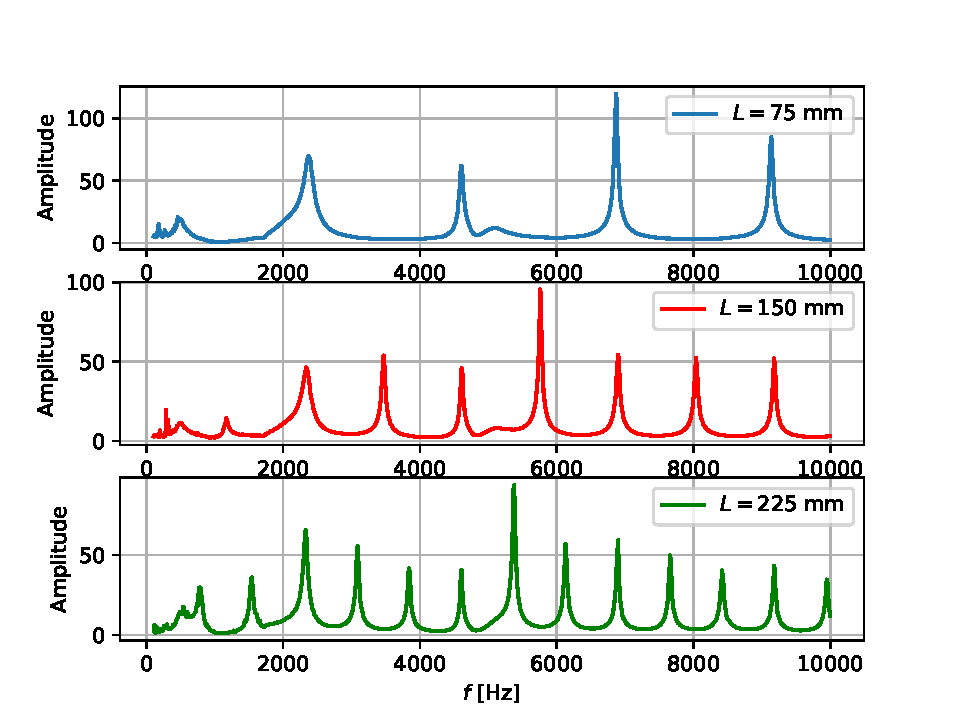
\includegraphics[scale=0.45]{Messwerte/plot1.pdf}
  \caption{Schallamplitude in verschieden langen Röhren $L$ bei variierender Frequenz.}
  \label{fig:plot1}
\end{figure}
\begin{figure}
  \centering
  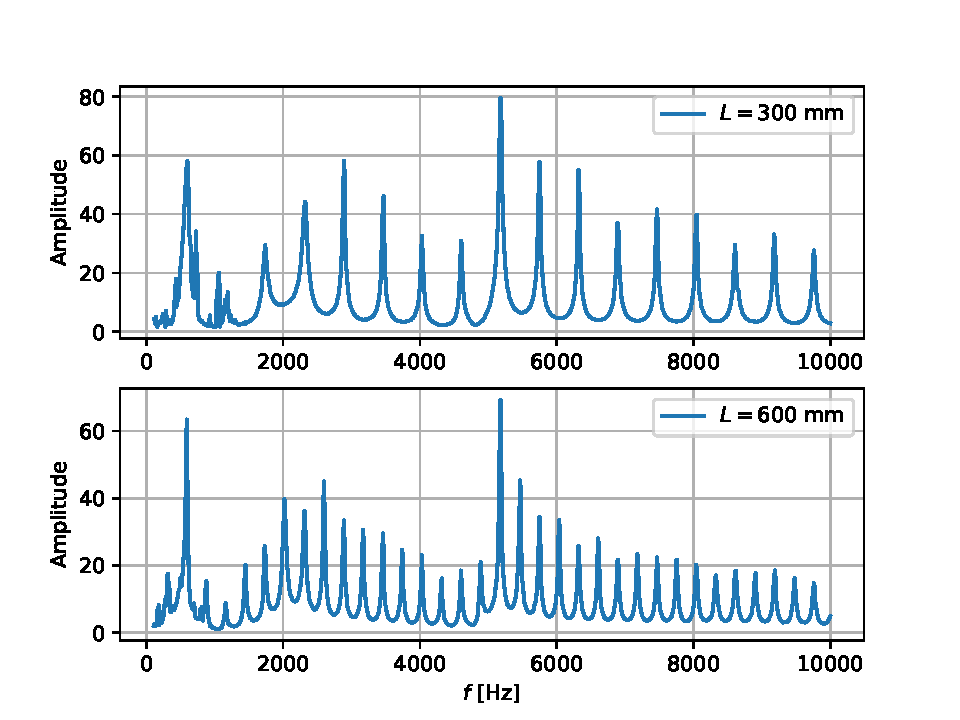
\includegraphics[scale=0.45]{Messwerte/plot2.pdf}
  \caption{Schallamplitude in verschieden langen Röhren $L$ bei variierender Frequenz.}
  \label{fig:plot2}
\end{figure}
Resonanzen treten auf, wenn die Bedingung
\begin{equation}
  2\cdot L=\frac{n\cdot c}{f}
\end{equation}
erfüllt ist. Dabei ist $L$ die Länge der Röhre, $n$ eine Natürliche Zahl, $c$ die Schallgeschwindigkeit und $f$ die Frequenz.
Umgestellt nach $f$:
\begin{equation}
  \underbrace{f}_{y}=\underbrace{\frac{c}{2\cdot L}}_{m}\underbrace{\cdot n}_{x}+\underbrace{0}_{b}.
\end{equation}
Die Steigung $m$ der Linearen Regression entspricht somit $\frac{c}{2\cdot L}$. Aufgelöst nach $c$ ergibt sich damit:
\begin{equation}
  c=m\cdot2\cdot L.
\end{equation}
Da $m$ fehlerbehaftet ist, muss der Ausdruck nach $m$ abgeleitet werden:
\begin{equation}
  \frac{\partial c}{\partial m}=2\cdot L.
\end{equation}
\begin{figure}
  \centering
  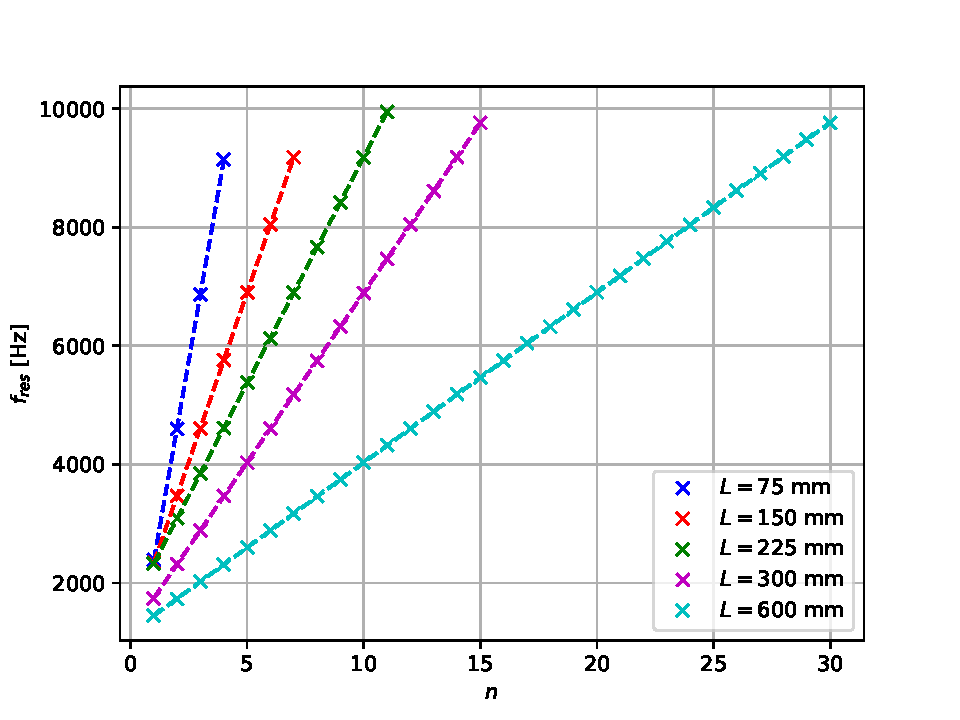
\includegraphics[scale=0.45]{Messwerte/plot3.pdf}
  \caption{Resonanzfrequenzen für Schallwellen bei verschieden Langen Röhren $L$ sowie die entsprechende Lineare Regression.}
  \label{fig:plot3}
\end{figure}
Eingesetzt in die Fehlerentwicklung nach Gauß:
\begin{align}
  \increment c &= \sqrt{\sum_i (\frac{\partial c}{\partial x_i}\cdot\increment x_i)^2}\\
  \increment c &= 2\cdot L\cdot\increment m
\end{align}
Die Steigungen der Linearen Regression $m$, sowie die daraus bestimmte Schallgeschwindigkeit $c$
der verschiedenen Längen $L$ sind in Tabelle \ref{tab:tab1} zu finden.
\begin{table}
  \centering
  \caption{Steigung der Linearen Regression $m$ der Resonanzfrequenzen aufgetragen gegen
  den Index $n$ bei verschiedenen Längen $L$, sowie die daraus berechnete Schallgeschwindigkeit $c$.}
  \label{tab:tab1}
  \begin{tabular}{c|c|c|c|c}
    $L \:/\: \si{\milli\meter}$ & $m \:/\: \si{\hertz}$ & $\increment m \:/\: \si{\hertz}$ & $c \:/\: \si{\meter\per\second}$ & $\increment c \:/\: \si{\meter\per\second}$ \\
    \midrule
    75 & 2252.0 & 10.39 & 337.80 & 1.60 \\
    150 & 1141.1 & 0.89 & 342.32 & 0.27 \\
    225 & 762.0 & 0.48 & 342.90 & 0.22 \\
    300 & 572.4 & 0.30 & 343.41 & 0.18 \\
    600 & 286.7 & 0.07 & 344.06 & 0.09
  \end{tabular}
\end{table}
Der gemittelte Wert für die Schallgeschwindigkeit, welcher sich nach
\begin{equation}
  \overline{x}=\frac{1}{N}\cdot\sum_{i=1}^{N}x_i
\end{equation}
bestimmt, beträgt $c=(342.098\pm 2.22)\si{\meter\per\second}$. Der angegebene Fehler ist
die Standardabweichung, welche nach
\begin{equation}
  \sigma = \overline{x^2}-\overline{x}^2
\end{equation}
bestimmt wurde. Verglichen mit dem Literaturwert von $\SI{343}{\meter\per\second}$
ergibt sich eine Abweichung von  %http://hyperphysics.phy-astr.gsu.edu/hbase/Tables/Soundv.html
\begin{align}
  p =& (\frac{c_{\text{Exp}}}{c_{\text{Lit}}}-1)\cdot100\\
  p =& -0.26\%.
\end{align}
Für $12$ $\SI{50}{\milli\meter}$ ist das Spektrum in Abbildung \ref{fig:plot4} abgebildet. Die Frequenz
ist in Abbildung \ref{fig:plot5} gegen die Wellenzahl $k$ aufgetragen.
\begin{figure}
  \centering
  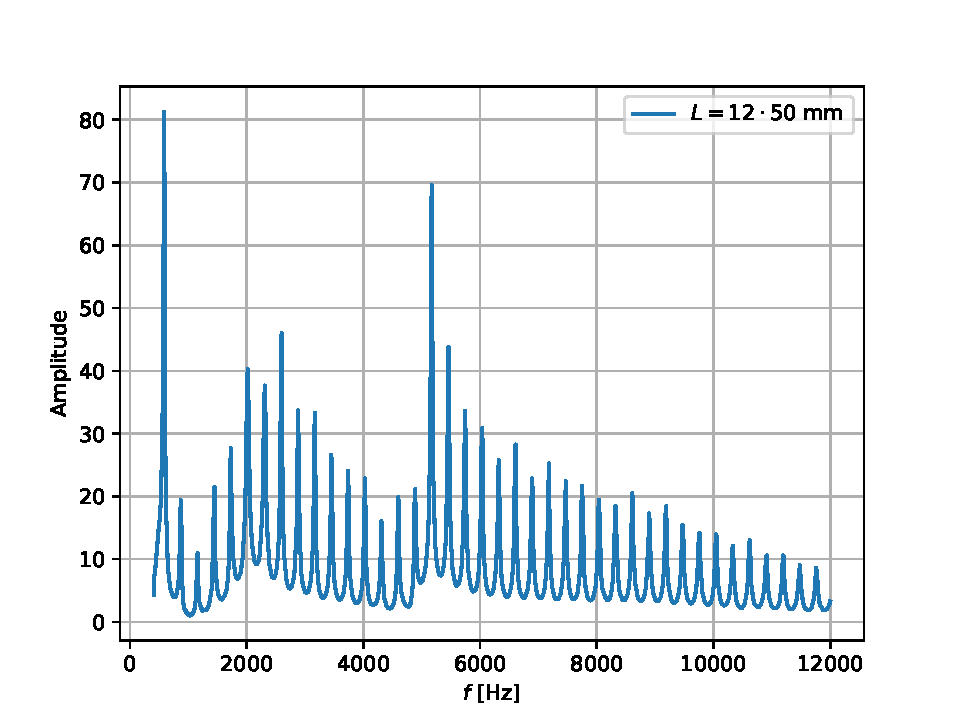
\includegraphics[scale=0.45]{Messwerte/plot4.pdf}
  \caption{Spektrum von einer Röhre, bestehend aus $12$ $\SI{50}{\milli\meter}$ langen Partien.}
  \label{fig:plot4}
\end{figure}
\begin{figure}
  \centering
  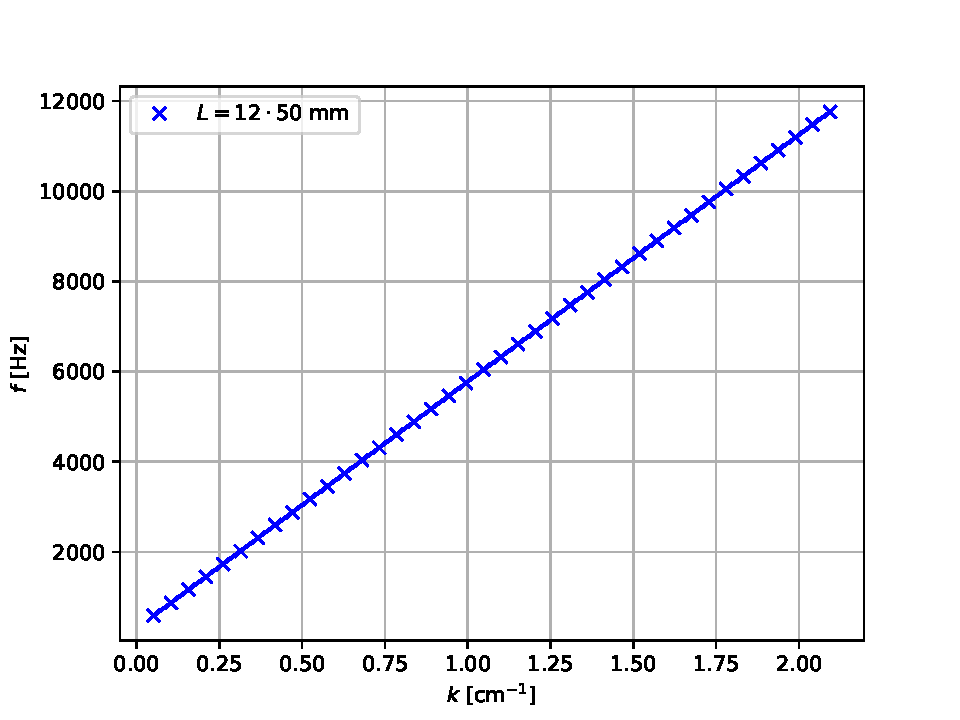
\includegraphics[scale=0.45]{Messwerte/plot5.pdf}
  \caption{Frequenzspektrum aufgetragen gegen die Wellenzahl $k$ für $12$ $\SI{50}{\milli\meter}$ Röhren.}
  \label{fig:plot5}
\end{figure}
Die Wellenzahl $k$ wird mit
\begin{equation}
  k=\frac{2\cdot\pi\cdot n}{L}
\end{equation}
bestimmt. Es wird an der Abbildung deutlich, dass es ein lineares Verhältnis $f(k)=d\cdot k$ sichtbar. Der Fitparameter für die Dispersion beträgt $d=5473.63$.
Somit ist die Dispersionsrelation $f(k)=5473.63\cdot k$.
\begin{figure}
  \centering
  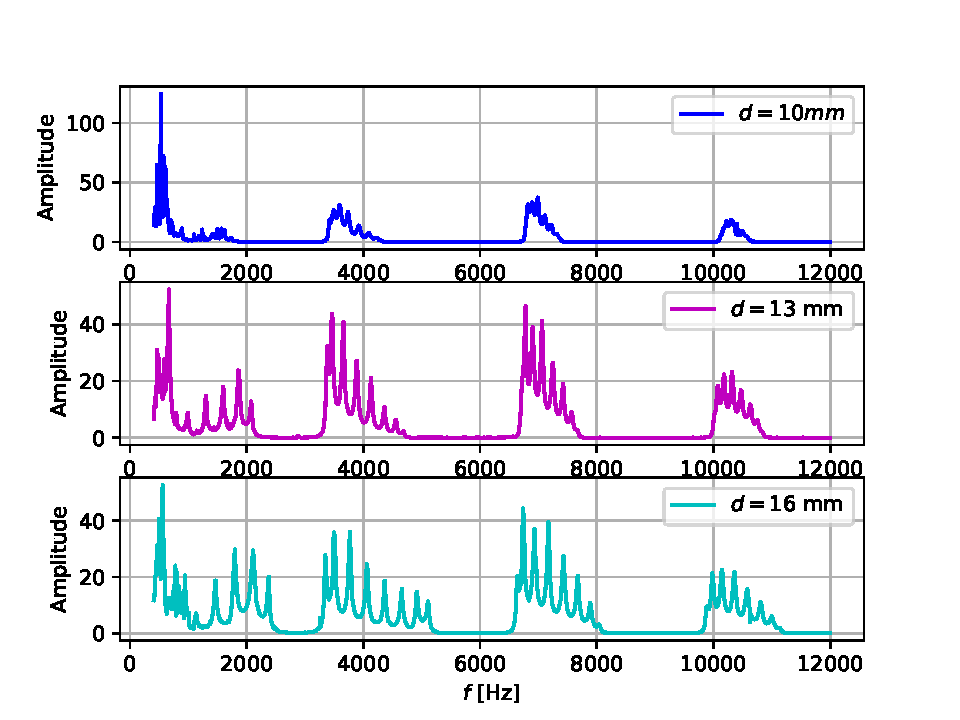
\includegraphics[scale=0.5]{Messwerte/plot6.pdf}
  \caption{Spektrum einer Röhre mit variierendem Durchmesser der Iris zwischen den Rohrabschnitten.}
  \label{fig:plot6}
\end{figure}
\begin{figure}
  \centering
  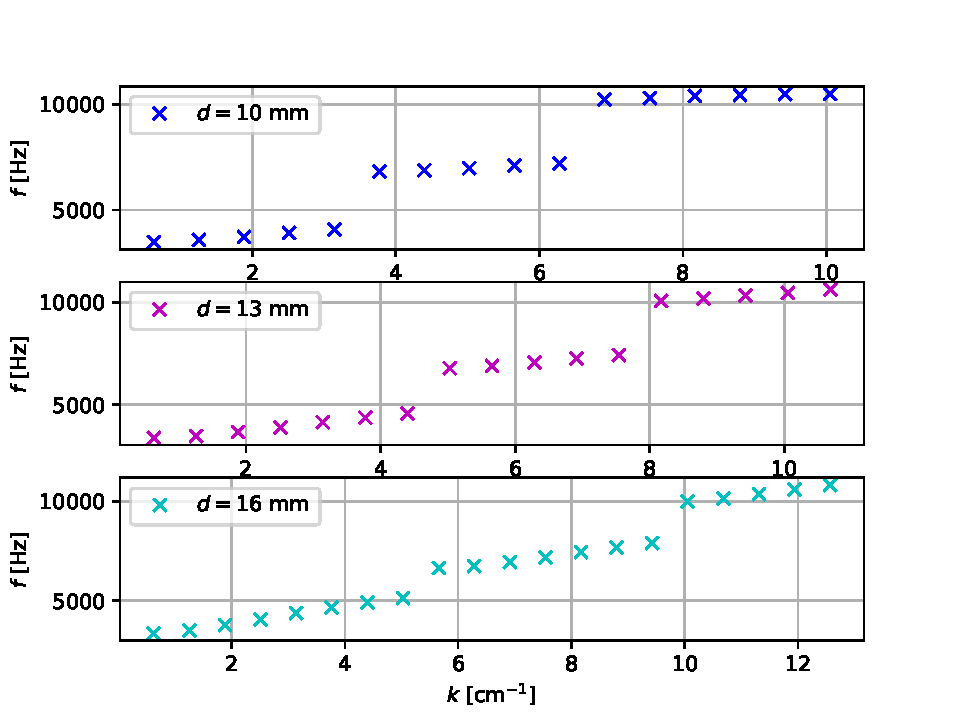
\includegraphics[scale=0.5]{Messwerte/plot7.pdf}
  \caption{Frequenz einer Röhre mit variierendem Durchmesser der Iris zwischen den Rohrabschnitten abhängig von der Wellenzahl $k$.}
  \label{fig:plot7}
\end{figure}
Aus Abbildung \ref{fig:plot7} wird deutlich, dass die Bänder mit steigendem Irisdurchmesser $d$ auch breiter werden.
\begin{figure}
  \centering
  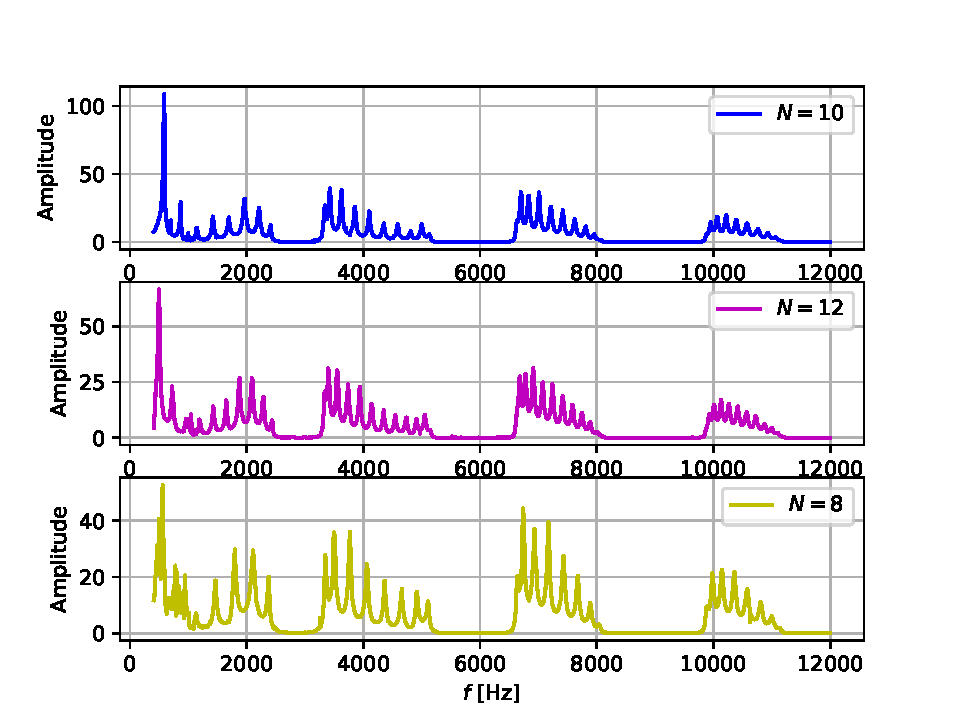
\includegraphics[scale=0.5]{Messwerte/plot8.pdf}
  \caption{Spektren von $n\cdot\SI{50}{\milli\meter}$ Röhren und einem Irisdurchmesser von $d=\SI{16}{\milli\meter}$.}
  \label{fig:plot8}
\end{figure}
Der Vergleich zwischen verschieden Langen Röhren mit einem Irisdurchmesser von $\SI{16}{\milli\meter}$ ist in Abbildung \ref{fig:plot8} zu sehen.
Die Amplitude wird für kleinere Rohrlängen größer, die Resonanzen scheinen bei gleicher Frequenz zu liegen.
\begin{figure}
  \centering
  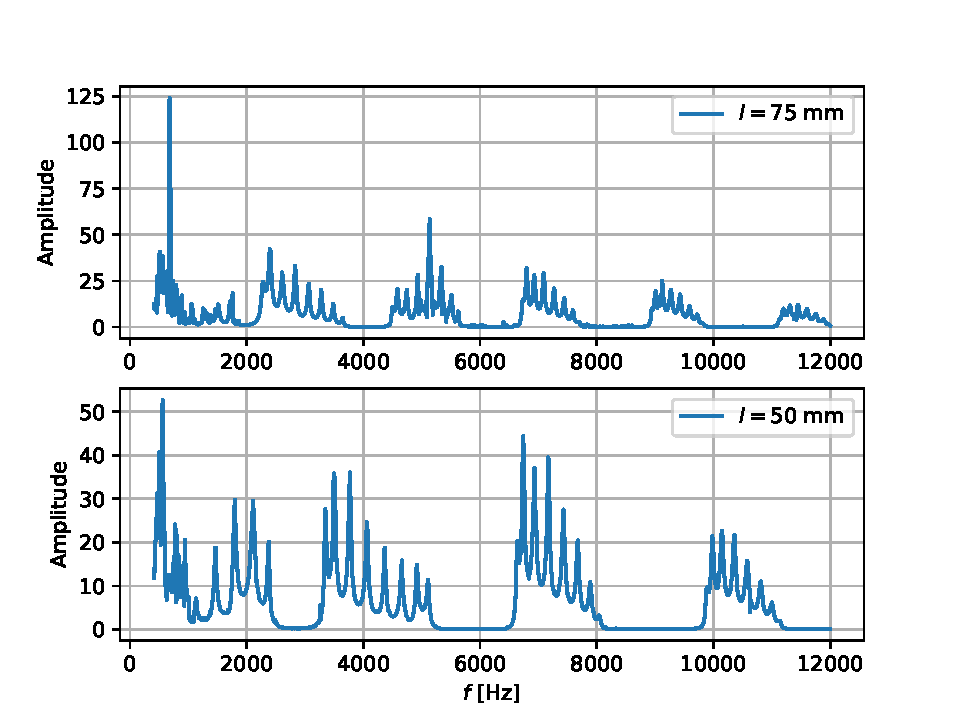
\includegraphics[scale=0.5]{Messwerte/plot9.pdf}
  \caption{Spektren von Röhren, bestehend aus $8$ Stücken mit der Länge $l$ und dem Irisdurchmesser $d=\SI{16}{\milli\meter}$.}
  \label{fig:plot9}
\end{figure}
Beim Vergleich der Spektren für $8$ einzelröhren mit der Länge $l=\SI{50}{\milli\meter}$ und $\SI{75}{\milli\meter}$ (Abbildung \ref{fig:plot9}) fällt auf, dass die
Amplitude bei kleineren Rohrlängen zunimmt und die Resonanzfrequenzen sich verschieben.

%\section{Diskussion}
Der experimentell bestimmte Wert für die Schallgeschwindigkeit
$c=\SI{342.098}{\meter\per\second}$ weicht nur $0,26\%$ vom Literaturwert ab,
was eine ziemlich präzise Messung darstellt.\\
Abbildungen \ref{fig:plot1}, \ref{fig:plot2}, \ref{fig:plot4} und \ref{fig:plot10} zeigen gut die Analogie
zwischen den Röhren und dem Quantenmechanischen Potentialtopf, welcher
nur diskrete Werte als Eigenenergie zulässt. Die Resonanzfrequenzen sind
diskret und deren Anzahl nimmt mit zunehmender Länge der Röhre zu.\\
In Abbildung \ref{fig:plot6}, \ref{fig:plot12}, \ref{fig:plot13}, \ref{fig:plot14} und \ref{fig:plot11} ist gut zu sehen, wie sich eine Welle bzw. die Wellenfunktion
eines Elektrons verhält, wenn es an einem hindernis mit variierendem Wirkungsquerschnitt
gestreut wird verhält, simuliert mit Iriden zwischen den Rohrabschnitten mit verschiedenen
durchmessern. Die Bandstrukturen in Abbildung \ref{fig:plot7} und \ref{fig:plot15}, welche aus der Streuung
resultieren zeigen die Energieniveaus des Elektrons.\\
Die Anzahl der Resonanzen pro Band nimmt mit steigender Anzahl von Elementarzellen
(simuliert mit $\SI{50}{\milli\meter}$ Röhren) zu, wie in Abbildung \ref{fig:plot8} zu sehen ist.\\
Der Einfluss des Raumes zwischen den Atomen, kann mit verschieden langen Rohren zwischen den
Iriden beeinflusst werden: Die Resonanzfrequenzen verschieben sich, während die
Anzahl der Maxima bleibt gleich (Abbildung \ref{fig:plot9}).\\
Ein Molekül, bestehend aus $2$ Atomen, wurde in Abbildung \ref{fig:plot16} simuliert mit alternierenden Iridendurchmesser (Wirkungsquerschnitt).
Verglichen mit einem Spektrum mit einem konstanten Irisdurchmesser wird deutlich, wie sich die Resonanzfrequenzen und damit
auch die Bandstrukturen aufspalten in Zwischenstufen, was in Abbildung \ref{fig:plot17} anschaulich dargestellt wird.\\
Der Einbau eines Defekts führte zu einer Störung der Bandstruktur, was zur bildung
eines neuen Zustands führt (Abbildung \ref{fig:plot18} und \ref{fig:plot19}).\\
Die nutzung von Schallwellen als Analogon zur Wellenfunktion eines Elektrons eignet sich gut,
um das Verhalten eines jenen Elektrons in einem Gitter oder Potentialtopfes zu untersuchen.

\printbibliography{}
\end{document}
